
\begin{frame}{Problem Description}
    Implement an Artificial Inteligence agent based on heuristic search methods to solve \href{https://erich-friedman.github.io/puzzle/robot/}{Robot Mazes} puzzle. 

    \vspace{0.5em}

    \begin{minipage}{0.62\textwidth}
        \begin{itemize}
            \item \textbf{Grid:} The puzzle is made up of a 5x5 grid, with a start and finish positions. Between each spot in the grid, there can be a wall.
            \item \textbf{Robot and Movement:} The robot is placed at the starting spot and can make a limited number of movements (Left, Right, Up or Down), depending on the puzzle. When there are no moves left, he will repeat the sequence chosen until he gets stuck or reaches the ending spot.
        \end{itemize}
    \end{minipage}%
    \begin{minipage}{0.38\textwidth}
        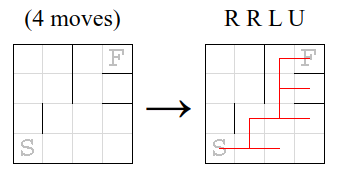
\includegraphics[width=50mm]{img/puzzle.png}
    \end{minipage}
    \begin{itemize}
            \item \textbf{Objective:} The objective is to, for a given puzzle, decide the correct sequence of movements for the robot to loop from start to finish.
    \end{itemize}
\end{frame}
